\documentclass[12pt]{report}\usepackage[]{graphicx}\usepackage[dvipsnames]{xcolor}
% maxwidth is the original width if it is less than linewidth
% otherwise use linewidth (to make sure the graphics do not exceed the margin)
\makeatletter
\def\maxwidth{ %
  \ifdim\Gin@nat@width>\linewidth
    \linewidth
  \else
    \Gin@nat@width
  \fi
}
\makeatother

\definecolor{fgcolor}{rgb}{0.345, 0.345, 0.345}
\newcommand{\hlnum}[1]{\textcolor[rgb]{0.686,0.059,0.569}{#1}}%
\newcommand{\hlstr}[1]{\textcolor[rgb]{0.192,0.494,0.8}{#1}}%
\newcommand{\hlcom}[1]{\textcolor[rgb]{0.678,0.584,0.686}{\textit{#1}}}%
\newcommand{\hlopt}[1]{\textcolor[rgb]{0,0,0}{#1}}%
\newcommand{\hlstd}[1]{\textcolor[rgb]{0.345,0.345,0.345}{#1}}%
\newcommand{\hlkwa}[1]{\textcolor[rgb]{0.161,0.373,0.58}{\textbf{#1}}}%
\newcommand{\hlkwb}[1]{\textcolor[rgb]{0.69,0.353,0.396}{#1}}%
\newcommand{\hlkwc}[1]{\textcolor[rgb]{0.333,0.667,0.333}{#1}}%
\newcommand{\hlkwd}[1]{\textcolor[rgb]{0.737,0.353,0.396}{\textbf{#1}}}%
\let\hlipl\hlkwb

\usepackage{framed}
\makeatletter
\newenvironment{kframe}{%
 \def\at@end@of@kframe{}%
 \ifinner\ifhmode%
  \def\at@end@of@kframe{\end{minipage}}%
  \begin{minipage}{\columnwidth}%
 \fi\fi%
 \def\FrameCommand##1{\hskip\@totalleftmargin \hskip-\fboxsep
 \colorbox{shadecolor}{##1}\hskip-\fboxsep
     % There is no \\@totalrightmargin, so:
     \hskip-\linewidth \hskip-\@totalleftmargin \hskip\columnwidth}%
 \MakeFramed {\advance\hsize-\width
   \@totalleftmargin\z@ \linewidth\hsize
   \@setminipage}}%
 {\par\unskip\endMakeFramed%
 \at@end@of@kframe}
\makeatother

\definecolor{shadecolor}{rgb}{.97, .97, .97}
\definecolor{messagecolor}{rgb}{0, 0, 0}
\definecolor{warningcolor}{rgb}{1, 0, 1}
\definecolor{errorcolor}{rgb}{1, 0, 0}
\newenvironment{knitrout}{}{} % an empty environment to be redefined in TeX

\usepackage{alltt}

\usepackage[utf8]{inputenc}
\usepackage[spanish]{babel}
\usepackage[margin=2.54cm]{geometry}
\usepackage[dvipsnames]{xcolor}
\usepackage{array, amssymb, amsthm, enumitem, fancyhdr, float, graphicx, hyperref, hologo, mathtools, tikz, tikz-cd}
\usepackage[spanish, noabbrev]{cleveref}

\pagestyle{fancy}
\lhead{\footnotesize \leftmark}
\rhead{\footnotesize \rightmark}

\title{
	\huge
	\noindent\textbf{Fundamentos de la Ciencia de Datos}\\
	
	{\Large \textit{Práctica 1}}
	\vspace{1cm}
	
	\huge
	Grado en Ingeniería Informática\\
	Universidad de Alcalá\\
	
	\vspace{1cm}
	
	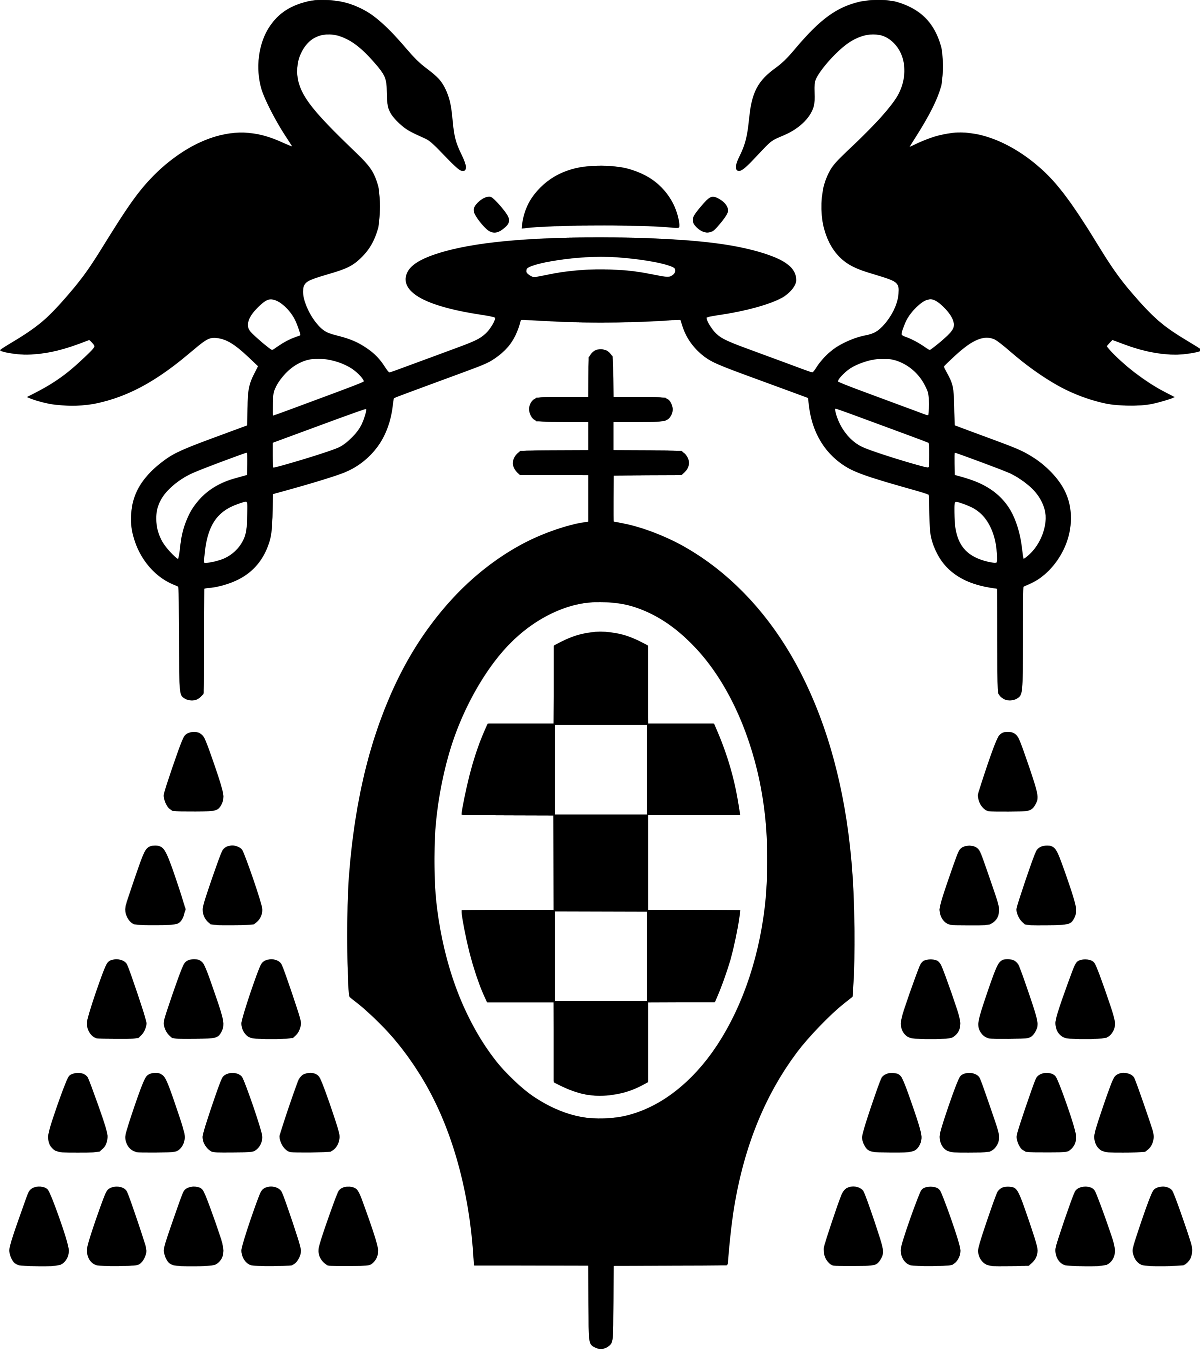
\includegraphics[scale=0.075]{img/logo}
}

\author{
	Pablo García García\\
	Abel López Martínez\\
	Álvaro Jesús Martínez Parra\\
	Raúl Moratilla Núñez
}

\date{
	\large{14 de noviembre de 2023}
}

\hypersetup{
	pdftitle={Práctica 1}, 
	pdfauthor={Pablo García García, Abel López Martínez, Álvaro Jesús Martínez Parra, Raúl Moratilla Núñez}, 
	pdfsubject={Fundamentos de la Ciencia de Datos}, 
	pdfcenterwindow, 
	pdfnewwindow=true, 
	pdfkeywords={Entrega de la PL1 de laboratorio correspondiente al Curso 2023-2024}, 
	bookmarksopen=true 
}
\IfFileExists{upquote.sty}{\usepackage{upquote}}{}
\begin{document}
	
\begin{knitrout}
\definecolor{shadecolor}{rgb}{0.969, 0.969, 0.969}\color{fgcolor}\begin{kframe}
\begin{alltt}
\hlstd{fichero} \hlkwb{=} \hlkwd{read.csv2}\hlstd{(}\hlstr{"prueba.csv"}\hlstd{)}

\hlstd{len} \hlkwb{=} \hlkwa{function}\hlstd{(}\hlkwc{list}\hlstd{)\{}
        \hlstd{count} \hlkwb{=} \hlnum{0}
        \hlkwa{for} \hlstd{(element} \hlkwa{in} \hlstd{list)\{}
                \hlstd{count} \hlkwb{=} \hlstd{count} \hlopt{+} \hlnum{1}
        \hlstd{\}}
        \hlstd{count}
\hlstd{\}}

\hlstd{distancias} \hlkwb{=} \hlstd{fichero}\hlopt{$}\hlstd{Numeros}

\hlkwd{len}\hlstd{(distancias)}
\end{alltt}
\begin{verbatim}
## [1] 12
\end{verbatim}
\begin{alltt}
\hlstd{bubble} \hlkwb{=} \hlkwa{function}\hlstd{(}\hlkwc{list}\hlstd{)\{}
        \hlstd{n} \hlkwb{=} \hlkwd{len}\hlstd{(list)}
        \hlkwa{for} \hlstd{(i} \hlkwa{in} \hlnum{2}\hlopt{:}\hlstd{n)\{}
                \hlkwa{for} \hlstd{(j} \hlkwa{in} \hlnum{1}\hlopt{:}\hlstd{(n}\hlopt{-}\hlnum{1}\hlstd{))\{}
                        \hlkwa{if} \hlstd{(list[j]} \hlopt{>} \hlstd{list[j}\hlopt{+}\hlnum{1}\hlstd{])\{}
                                \hlstd{temp} \hlkwb{=} \hlstd{list[j]}
                                \hlstd{list[j]} \hlkwb{=} \hlstd{list[j}\hlopt{+}\hlnum{1}\hlstd{]}
                                \hlstd{list[j}\hlopt{+}\hlnum{1}\hlstd{]} \hlkwb{=} \hlstd{temp}
                        \hlstd{\}}
                \hlstd{\}}
        \hlstd{\}}
        \hlstd{list}
\hlstd{\}}
\hlstd{distanciasordenadas} \hlkwb{=} \hlkwd{bubble}\hlstd{(distancias)}
\hlstd{distanciasordenadas}
\end{alltt}
\begin{verbatim}
##  [1] 13 15 16 20 20 22 27 29 30 33 34 42
\end{verbatim}
\begin{alltt}
\hlstd{rank} \hlkwb{=} \hlkwa{function}\hlstd{(}\hlkwc{list}\hlstd{)\{}
        \hlstd{ordered_list} \hlkwb{=} \hlkwd{bubble}\hlstd{(list)}
        \hlstd{ordered_list[}\hlkwd{len}\hlstd{(ordered_list)]} \hlopt{-} \hlstd{ordered_list[}\hlnum{1}\hlstd{]}
\hlstd{\}}

\hlstd{rango} \hlkwb{=} \hlkwd{rank}\hlstd{(distanciasordenadas)}
\hlstd{rango}
\end{alltt}
\begin{verbatim}
## [1] 29
\end{verbatim}
\begin{alltt}
\hlstd{absolute_freq} \hlkwb{=} \hlkwa{function}\hlstd{(}\hlkwc{list}\hlstd{)\{}
        \hlstd{ordered_list} \hlkwb{=} \hlkwd{bubble}\hlstd{(list)}
        \hlstd{n} \hlkwb{=} \hlkwd{len}\hlstd{(ordered_list)}
        \hlstd{elements} \hlkwb{=} \hlkwd{vector}\hlstd{()}
        \hlstd{frequencies} \hlkwb{=} \hlkwd{vector}\hlstd{()}
        \hlstd{i} \hlkwb{=} \hlnum{1}
        \hlkwa{while} \hlstd{(i} \hlopt{<=} \hlstd{n)\{}
                \hlstd{actual_element} \hlkwb{=} \hlstd{ordered_list[i]}
                \hlstd{elements} \hlkwb{=} \hlkwd{append}\hlstd{(elements, actual_element)}
                \hlstd{actual_freq} \hlkwb{=} \hlnum{0}
                \hlstd{j} \hlkwb{=} \hlstd{i}
                \hlkwa{while}\hlstd{(j} \hlopt{<=} \hlstd{n} \hlopt{&} \hlstd{actual_element} \hlopt{==} \hlstd{ordered_list[j])\{}
                        \hlstd{actual_freq} \hlkwb{=} \hlstd{actual_freq} \hlopt{+} \hlnum{1}
                        \hlstd{j} \hlkwb{=} \hlstd{j}\hlopt{+}\hlnum{1}
                \hlstd{\}}
                \hlstd{frequencies} \hlkwb{=} \hlkwd{append}\hlstd{(frequencies, actual_freq)}
                \hlstd{i} \hlkwb{=} \hlstd{j}
        \hlstd{\}}
        \hlkwd{rbind}\hlstd{(elements, frequencies)}
\hlstd{\}}
\hlstd{frecuencia_abs} \hlkwb{=} \hlkwd{absolute_freq}\hlstd{(distancias)}
\hlstd{frecuencia_abs}
\end{alltt}
\begin{verbatim}
##             [,1] [,2] [,3] [,4] [,5] [,6] [,7] [,8] [,9] [,10] [,11]
## elements      13   15   16   20   22   27   29   30   33    34    42
## frequencies    1    1    1    2    1    1    1    1    1     1     1
\end{verbatim}
\begin{alltt}
\hlstd{relative_freq} \hlkwb{=} \hlkwa{function}\hlstd{(}\hlkwc{list}\hlstd{)\{}
        \hlstd{f_abs} \hlkwb{=} \hlkwd{absolute_freq}\hlstd{(list)}
        \hlstd{elements} \hlkwb{=} \hlstd{f_abs[}\hlnum{1}\hlstd{,]}
        \hlstd{abs_fvalues} \hlkwb{=} \hlstd{f_abs[}\hlnum{2}\hlstd{,]}
        \hlkwd{rbind}\hlstd{(elements,abs_fvalues}\hlopt{/}\hlkwd{len}\hlstd{(list))}
\hlstd{\}}

\hlstd{frecuencia_rel} \hlkwb{=} \hlkwd{relative_freq}\hlstd{(distancias)}
\hlstd{frecuencia_rel}
\end{alltt}
\begin{verbatim}
##                 [,1]        [,2]        [,3]       [,4]        [,5]        [,6]
## elements 13.00000000 15.00000000 16.00000000 20.0000000 22.00000000 27.00000000
##           0.08333333  0.08333333  0.08333333  0.1666667  0.08333333  0.08333333
##                 [,7]        [,8]        [,9]       [,10]       [,11]
## elements 29.00000000 30.00000000 33.00000000 34.00000000 42.00000000
##           0.08333333  0.08333333  0.08333333  0.08333333  0.08333333
\end{verbatim}
\begin{alltt}
\hlstd{acum_absolute_freq} \hlkwb{=} \hlkwa{function}\hlstd{(}\hlkwc{list}\hlstd{)\{}
        \hlstd{f_abs} \hlkwb{=} \hlkwd{absolute_freq}\hlstd{(list)}
        \hlstd{elements} \hlkwb{=} \hlstd{f_abs[}\hlnum{1}\hlstd{,]}
        \hlstd{abs_fvalues} \hlkwb{=} \hlstd{f_abs[}\hlnum{2}\hlstd{,]}
        \hlstd{acum_abs_fvalues} \hlkwb{=} \hlkwd{vector}\hlstd{()}
        \hlstd{acum} \hlkwb{=} \hlnum{0}
        \hlkwa{for} \hlstd{(i} \hlkwa{in} \hlnum{1}\hlopt{:}\hlkwd{len}\hlstd{(elements))\{}
                \hlstd{acum} \hlkwb{=} \hlstd{acum} \hlopt{+} \hlstd{abs_fvalues[i]}
                \hlstd{acum_abs_fvalues} \hlkwb{=} \hlkwd{append}\hlstd{(acum_abs_fvalues, acum)}
        \hlstd{\}}
        \hlkwd{rbind}\hlstd{(elements, acum_abs_fvalues)}
\hlstd{\}}
\hlstd{frecuencia_abs_acum} \hlkwb{=} \hlkwd{acum_absolute_freq}\hlstd{(distancias)}
\hlstd{frecuencia_abs_acum}
\end{alltt}
\begin{verbatim}
##                  [,1] [,2] [,3] [,4] [,5] [,6] [,7] [,8] [,9] [,10] [,11]
## elements           13   15   16   20   22   27   29   30   33    34    42
## acum_abs_fvalues    1    2    3    5    6    7    8    9   10    11    12
\end{verbatim}
\begin{alltt}
\hlstd{acum_relative_freq} \hlkwb{=} \hlkwa{function}\hlstd{(}\hlkwc{list}\hlstd{)\{}
        \hlstd{f_rel} \hlkwb{=} \hlkwd{relative_freq}\hlstd{(list)}
        \hlstd{elements} \hlkwb{=} \hlstd{f_rel[}\hlnum{1}\hlstd{,]}
        \hlstd{rel_fvalues} \hlkwb{=} \hlstd{f_rel[}\hlnum{2}\hlstd{,]}
        \hlstd{acum_rel_fvalues} \hlkwb{=} \hlkwd{vector}\hlstd{()}
        \hlstd{acum} \hlkwb{=} \hlnum{0}
        \hlkwa{for} \hlstd{(i} \hlkwa{in} \hlnum{1}\hlopt{:}\hlkwd{len}\hlstd{(elements))\{}
                \hlstd{acum} \hlkwb{=} \hlstd{acum} \hlopt{+} \hlstd{rel_fvalues[i]}
                \hlstd{acum_rel_fvalues} \hlkwb{=} \hlkwd{append}\hlstd{(acum_rel_fvalues, acum)}
        \hlstd{\}}
        \hlkwd{rbind}\hlstd{(elements, acum_rel_fvalues)}
\hlstd{\}}
\hlstd{frecuencia_rel_acum} \hlkwb{=} \hlkwd{acum_relative_freq}\hlstd{(distancias)}
\hlstd{frecuencia_rel_acum}
\end{alltt}
\begin{verbatim}
##                         [,1]       [,2]  [,3]       [,4] [,5]       [,6]
## elements         13.00000000 15.0000000 16.00 20.0000000 22.0 27.0000000
## acum_rel_fvalues  0.08333333  0.1666667  0.25  0.4166667  0.5  0.5833333
##                        [,7]  [,8]       [,9]      [,10] [,11]
## elements         29.0000000 30.00 33.0000000 34.0000000    42
## acum_rel_fvalues  0.6666667  0.75  0.8333333  0.9166667     1
\end{verbatim}
\begin{alltt}
\hlstd{mean} \hlkwb{=} \hlkwa{function}\hlstd{(}\hlkwc{list}\hlstd{)\{}
        \hlstd{total} \hlkwb{=} \hlnum{0}
        \hlstd{n} \hlkwb{=} \hlkwd{len}\hlstd{(list)}
        \hlkwa{for} \hlstd{(i} \hlkwa{in} \hlnum{1}\hlopt{:}\hlstd{n)\{}
                \hlstd{total} \hlkwb{=} \hlstd{total} \hlopt{+} \hlstd{list[i]}
        \hlstd{\}}
        \hlstd{mean} \hlkwb{=} \hlstd{total} \hlopt{/} \hlstd{n}
        \hlstd{mean}
\hlstd{\}}

\hlstd{media} \hlkwb{=} \hlkwd{mean}\hlstd{(distancias)}
\hlstd{media}
\end{alltt}
\begin{verbatim}
## [1] 25.08333
\end{verbatim}
\begin{alltt}
\hlstd{mode} \hlkwb{=} \hlkwa{function}\hlstd{(}\hlkwc{list}\hlstd{)\{}
        \hlstd{frequencies} \hlkwb{=} \hlkwd{absolute_freq}\hlstd{(list)}
        \hlstd{elements} \hlkwb{=} \hlstd{frequencies[}\hlnum{1}\hlstd{,]}
        \hlstd{freq_values} \hlkwb{=} \hlstd{frequencies[}\hlnum{2}\hlstd{,]}
        \hlstd{actual_mode} \hlkwb{=} \hlnum{0}
        \hlstd{actual_mode_val} \hlkwb{=} \hlnum{0}
        \hlkwa{for} \hlstd{(i} \hlkwa{in} \hlnum{1}\hlopt{:}\hlkwd{len}\hlstd{(elements))\{}
                \hlkwa{if} \hlstd{(freq_values[i]} \hlopt{>} \hlstd{actual_mode_val)\{}
                        \hlstd{actual_mode_val} \hlkwb{=} \hlstd{freq_values[i]}
                        \hlstd{actual_mode} \hlkwb{=} \hlstd{elements[i]}
                \hlstd{\}}
        \hlstd{\}}
        \hlstd{actual_mode}
\hlstd{\}}

\hlstd{moda} \hlkwb{=} \hlkwd{mode}\hlstd{(distancias)}
\hlstd{moda}
\end{alltt}
\begin{verbatim}
## [1] 20
\end{verbatim}
\begin{alltt}
\hlstd{median} \hlkwb{=} \hlkwa{function}\hlstd{(}\hlkwc{list}\hlstd{)\{}
        \hlstd{n} \hlkwb{=} \hlkwd{len}\hlstd{(list)}
        \hlkwa{if} \hlstd{(n}\hlopt\hlnum{2} \hlopt{==} \hlnum{0}\hlstd{)\{}
                \hlstd{median} \hlkwb{=} \hlstd{(list[n}\hlopt{/}\hlnum{2}\hlstd{]} \hlopt{+} \hlstd{list[(n}\hlopt{/}\hlnum{2}\hlstd{)}\hlopt{+}\hlnum{1}\hlstd{])} \hlopt{/} \hlnum{2}
        \hlstd{\}}
        \hlkwa{else}\hlstd{\{}
                \hlstd{median} \hlkwb{=} \hlstd{list[(n}\hlopt{+}\hlnum{1}\hlstd{)}\hlopt{/}\hlnum{2}\hlstd{]}
        \hlstd{\}}
        \hlstd{median}
\hlstd{\}}

\hlstd{mediana} \hlkwb{=} \hlkwd{median}\hlstd{(distancias)}
\hlstd{mediana}
\end{alltt}
\begin{verbatim}
## [1] 24.5
\end{verbatim}
\begin{alltt}
\hlstd{standard_desv} \hlkwb{=} \hlkwa{function}\hlstd{(}\hlkwc{list}\hlstd{)\{}
        \hlstd{mean} \hlkwb{=} \hlkwd{mean}\hlstd{(list)}
        \hlstd{n} \hlkwb{=} \hlkwd{len}\hlstd{(list)}
        \hlstd{add} \hlkwb{=} \hlnum{0}
        \hlkwa{for} \hlstd{(i} \hlkwa{in} \hlnum{1}\hlopt{:}\hlstd{n)\{}
                \hlstd{add} \hlkwb{=} \hlstd{add} \hlopt{+} \hlstd{((list[i]} \hlopt{-} \hlstd{mean)}\hlopt{^}\hlnum{2}\hlstd{)}
        \hlstd{\}}
        \hlkwd{sqrt}\hlstd{(add}\hlopt{/}\hlstd{n)}
\hlstd{\}}

\hlstd{desviacion} \hlkwb{=} \hlkwd{standard_desv}\hlstd{(distancias)}
\hlstd{desviacion}
\end{alltt}
\begin{verbatim}
## [1] 8.47996
\end{verbatim}
\begin{alltt}
\hlstd{variance} \hlkwb{=} \hlkwa{function}\hlstd{(}\hlkwc{list}\hlstd{)\{}
        \hlstd{desv} \hlkwb{=} \hlkwd{standard_desv}\hlstd{(list)}
        \hlstd{var} \hlkwb{=} \hlstd{desv}\hlopt{^}\hlnum{2}
        \hlstd{var}
\hlstd{\}}

\hlstd{varianza} \hlkwb{=} \hlkwd{variance}\hlstd{(distancias)}
\hlstd{varianza}
\end{alltt}
\begin{verbatim}
## [1] 71.90972
\end{verbatim}
\begin{alltt}
\hlstd{quant} \hlkwb{=} \hlkwa{function}\hlstd{(}\hlkwc{list}\hlstd{,} \hlkwc{c}\hlstd{)\{}
        \hlstd{ordered_list} \hlkwb{=} \hlkwd{bubble}\hlstd{(list)}
        \hlstd{n} \hlkwb{=} \hlkwd{len}\hlstd{(list)}
        \hlkwa{if} \hlstd{(c} \hlopt{<} \hlnum{0}\hlstd{)\{}
                \hlstd{quant} \hlkwb{=} \hlnum{0}
        \hlstd{\}}
        \hlkwa{else}\hlstd{\{}
                \hlkwa{if}\hlstd{((n}\hlopt{*}\hlstd{c)}\hlopt\hlnum{1} \hlopt{==} \hlnum{0}\hlstd{)\{}
                        \hlstd{quant} \hlkwb{=} \hlstd{(ordered_list[(n}\hlopt{*}\hlstd{c)]} \hlopt{+} \hlstd{ordered_list[(n}\hlopt{*}\hlstd{c)} \hlopt{+} \hlnum{1}\hlstd{])} \hlopt{/} \hlnum{2}
                \hlstd{\}}
                \hlkwa{else} \hlstd{\{}
                        \hlstd{int_prod} \hlkwb{=} \hlkwd{floor}\hlstd{(n}\hlopt{*}\hlstd{c)}
                        \hlstd{quant} \hlkwb{=} \hlstd{ordered_list[int_prod} \hlopt{+} \hlnum{1}\hlstd{]}
                \hlstd{\}}
        \hlstd{\}}
        \hlstd{quant}
\hlstd{\}}

\hlstd{cuartil1} \hlkwb{=} \hlkwd{quant}\hlstd{(distancias,}\hlnum{0.25}\hlstd{)}
\hlstd{cuartil2} \hlkwb{=} \hlkwd{quant}\hlstd{(distancias,}\hlnum{0.5}\hlstd{)}
\hlstd{cuartil3} \hlkwb{=} \hlkwd{quant}\hlstd{(distancias,}\hlnum{0.75}\hlstd{)}
\hlstd{cuartil1}
\end{alltt}
\begin{verbatim}
## [1] 18
\end{verbatim}
\begin{alltt}
\hlstd{cuartil2}
\end{alltt}
\begin{verbatim}
## [1] 24.5
\end{verbatim}
\begin{alltt}
\hlstd{cuartil3}
\end{alltt}
\begin{verbatim}
## [1] 31.5
\end{verbatim}
\end{kframe}
\end{knitrout}
\end{document}          
